% Note that the a4paper option is mainly intended so that authors in
% countries using A4 can easily print to A4 and see how their papers will
% look in print - the typesetting of the document will not typically be
% affected with changes in paper size (but the bottom and side margins will).
% Use the testflow package mentioned above to verify correct handling of
% both paper sizes by the user's LaTeX system.
%
% Also note that the "draftcls" or "draftclsnofoot", not "draft", option
% should be used if it is desired that the figures are to be displayed in
% draft mode.
%
\documentclass[conference, compsoc, 12pt]{IEEEtran}
\usepackage{blindtext, graphicx}
\usepackage[portuguese]{babel}
\usepackage[utf8]{inputenc}
\usepackage{hyperref}
\usepackage{graphicx}



% correct bad hyphenation here
\hyphenation{op-tical net-works semi-conduc-tor}


\begin{document}
%
% paper title
% can use linebreaks \\ within to get better formatting as desired
\title{Reconhecimento de alumínio e outros metais em meio ao lixo utilizando a base de dados de matérias MINC}

\author{\IEEEauthorblockN{Renato Nobre}
\IEEEauthorblockA{15/0146698\\
Departamento de\\Ciência da Computação\\
Universidade de Brasília}
\and
\IEEEauthorblockN{Khalil Carsten}
\IEEEauthorblockA{15/0134495\\Departamento de\\Ciência da Computação\\
Universidade de Brasília}}

\maketitle


\IEEEpeerreviewmaketitle

\begin{abstract}

\end{abstract}


\section{Introdução}

O alumínio é o metal mais abundante na natureza e recentemente utilizado em diversas aplicações, como em embalagens, transmissões elétricas, construção civil e elementos estruturais de meios de transporte. O seu uso cada vez mais constante prova sua relevância para a vida moderna, e consequentemente cada vez mais haverá descartes intensos do material para o lixo. Portanto, facilitar sua reciclagem geraria maiores benefícios econômicos, sociais e políticos. De acordo com o artigo publicado na Folha de São Paulo o Brasil é o maior reciclador de latas de alumínio do mundo e que esta atividade de venda e reciclagem dessas latas injetaram cerca de 845 milhões de reais na economia.

Este trabalho propõe no entanto uma maneira de facilitar a identificação do alumínio e metais dentro de outros tipos de lixo. Porém percebe-se que o reconhecimento de metais em imagens de lixo do mundo real é uma tarefa desafiadora. Os materiais que podem conter no lixo contém uma diversa gama de textura, geometria, luminosidade e agrupamento, que combinados geram o problema particularmente difícil. Para tentar superar essa dificuldade, foi utilizado um conjunto de imagens em grande escala de materiais em diversos ambientes. Esse conjunto de imagens denominado, materiais em banco de dados de contexto, MINC (do inglês, \textit{Materials in Context Database}), foi criado no departamento de ciência da computação da Universidade de Cornell e possui mais de três milhões de figuras de imagens. O MINC tem sua magnitude de materiais mais ampla que os bancos de imagens anteriores e é bem separado em 23 categorias diversas.

Utilizamos a CNN já treinada pelo MINC disponibilizada pelos autores de \cite{Artigo principal} no site \href{http://opensurfaces.cs.cornell.edu/publications/minc/>}{OpenSurface}. No entanto, notou-se que o MINC possuía em quase todas as imagens de treinamento um material bem separado do fundo e centralizado na imagem. Além disso, as imagens de treinamento para metais, o nosso foco nesse projeto, resumiam-se em eletro-domésticos, pias de metal, aço inox, aparatos de cozinha no geral. Isso prejucou muito a análise de imagens de entulho de lixo onde os materiais mais comuns estão entre: latas de alimentos enlatados, eletrônicos e latas de refrigerante. Para contornar esse problema tivemos que executar um refinamento na CNN com imagens que coletamos do repositório \href{https://github.com/garythung/trashnet}{https://github.com/garythung/trashnet} em que o autor treinou uma CNN somente para reconhecimento de lixos.

Em resumo, este trabalho fornece duas contribuições:

\begin{enumerate}
    \item Uma forma de separar metais do resto do lixo utilizando o banco de imagens MINC com uma rede neural co-evolucionária que possui uma arquitetura AlexNet
    \item Métodos de analisar a imagem em segmentos menores na rede neural AlexNet
\end{enumerate}


\section{Modelo}

Ao realizar trabalhos de reconhecimento de imagens, um grande obstáculo é a construção de uma base consistente para
treinar um modelo de aprendizagem. Reconhecimento de materiais requer que uma grande quantidade de imagens de diversas classes
sejam separadas e utilizadas, para superar essa dificuldade foi utilizado o banco de imagens MINC.

O MINC foi utilizado devido ao fato de consistir de mais de três milhões de imagens, com 23 categorias de materiais diferentes;
seu tamanho é grande o suficiente para métodos de aprendizagem conseguir generalizar casos de teste; suas diversas categorias
são representadas todas por uma diversa quantidade de conteúdo; há diversidade da disposição do conteúdo analisado na imagem.

A construção do MINC usou como base uma banco de imagens já existente, o FMD (do inglês, \textit{Flickr Material Database}). No entanto,
precisava de mais conteudo para a criação de um banco de imagens consistente e para isso integrou fotos de um site contendo imagens
de fotos profissioais de design de interior.

Após a criação do MINC, os autores de \emph{Material Recognition in the Wild with the Materials in Context Database} utilizaram uma rede AlexNet
\cite{Artigo principal} para testar a eficiencia do seu banco de imagens na criação de um modelo de aprendizagem.
As fotos utilizadas do MINC foram dividas em casos de teste e treino e foram inseridas no modelo de forma como mostrado na \emph{Figura 1, 2, 3, 4}.
Consequentemente, como grande parte do MINC foi feito utilizando fotos de interior de casas, ao analisar que contém diversos materiais em grande quantidades,
como imagens de entulho ou sucata de lixo mostrado na \emph{Figura 5, 6, 7, 8} a rede perdia muita precisão. O excesso de materiais e a diferença de uniformidade
da textura e luminosidade geraram uma mudança significante na média de acerto da AlexNet.

\begin{figure}[ht]
  \label{fig2}
  \begin{minipage}[b]{0.5\linewidth}
    \centering
    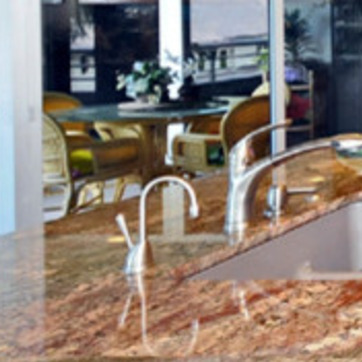
\includegraphics[width=.8\linewidth]{metal_000001.jpg}
    \caption{Metal 1}
    \vspace{4ex}
  \end{minipage}%%
  \begin{minipage}[b]{0.5\linewidth}
    \centering
    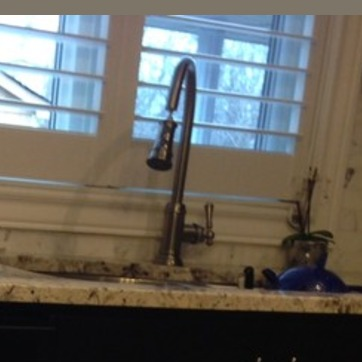
\includegraphics[width=.8\linewidth]{metal_000012.jpg}
    \caption{Metal 2}
    \vspace{4ex}
  \end{minipage}
  \begin{minipage}[b]{0.5\linewidth}
    \centering
    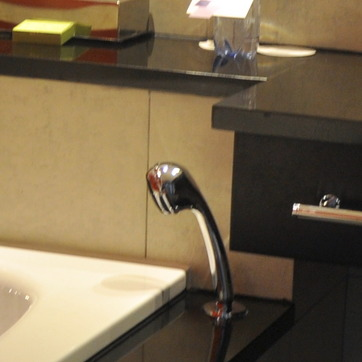
\includegraphics[width=.8\linewidth]{metal_000015.jpg}
    \caption{Metal 3}
    \vspace{4ex}
  \end{minipage}%%
  \begin{minipage}[b]{0.5\linewidth}
    \centering
    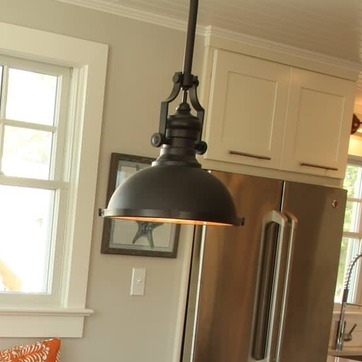
\includegraphics[width=.8\linewidth]{metal_000025.jpg}
    \caption{Metal 4}
    \vspace{4ex}
  \end{minipage}
\end{figure}


Torna-se evidente que ao analisarmos fotos de lixo com a AlexNet disponibilizada, a porcentagem de acerto dos matérias metálicos
reduz bastante. No entanto, como primeiro passo utilizamos de maneira simplista e direta a AlexNet pre-treinada,
para uma classificação de metais usando como entrada \emph{patchs}
de imagens com entulhos ou conjunto de materiais diversos. A \emph{Tabela 1}
mostra o resultado desta classificação. Não obteve nenhum acerto e notas bem baixas,
sendo $1$ a maior nota possível e tal nota dividida entre todas as 23 classes.
Portanto julgar uma imagem entre 23 possibilidade de classe se torna um tanto excessivo
quando o objetivo é somente julgar se algo é ou não um metal.

\begin{figure}[ht]
  \label{fig1}
  \begin{minipage}[b]{0.5\linewidth}
    \centering
    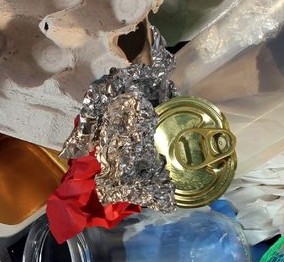
\includegraphics[width=.8\linewidth]{lixo1.jpg}
    \caption{Lixo 1}
    \vspace{4ex}
  \end{minipage}%%
  \begin{minipage}[b]{0.5\linewidth}
    \centering
    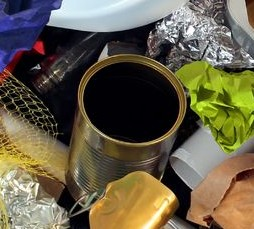
\includegraphics[width=.8\linewidth]{lixo2.jpg}
    \caption{Lixo 2}
    \vspace{4ex}
  \end{minipage}
  \begin{minipage}[b]{0.5\linewidth}
    \centering
    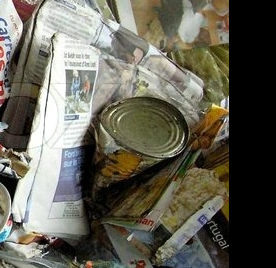
\includegraphics[width=.8\linewidth]{lixo3.png}
    \caption{Lixo 3}
    \vspace{4ex}
  \end{minipage}%%
  \begin{minipage}[b]{0.5\linewidth}
    \centering
    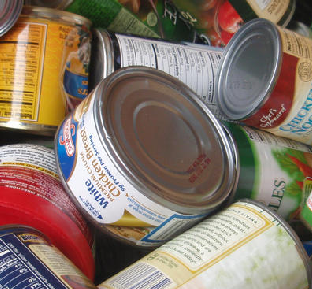
\includegraphics[width=.8\linewidth]{lixo4.png}
    \caption{Lixo 4}
    \vspace{4ex}
  \end{minipage}
\end{figure}

\begin{table}[]
\centering
\caption{Classificação AlexNet MINC}
\label{Tabela 1}
\begin{tabular}{|l|l|l|}
\hline
Imagens & Resultado & Nota \\ \hline
Lixo 1 & Vidro & $0.0755$ \\ \hline
Lixo 2 & Papel de Parede & $0.0040$ \\ \hline
Lixo 3 & Papel de Parede & $0.0096$\\ \hline
Lixo 4 & Espelho & $0.0316$ \\ \hline
\end{tabular}
\end{table}

\section{Solução e Análise}

Tendo em vista que o objetivo é analisar

\section{Resultados}

Para testar a solução proposta para o problema na seção anterior foram realizados diversos experimentos, com o objetivo de abranger todo o escopo do problema e analisar individualmente cada uma das implementações realizadas. Os experimentos foram realizados da forma que se descreve a seguir:

\begin{itemize}
    \item Um experimento realizado com a AlexNet sem nenhuma modificação, do jeito fornecido pelo artigo \cite{Artigo principal}. Com esse experimento podemos usar de base para comparar o efeito das modificações feitas.
    \item Um experimento realizado com a AlexNet refinada com a base de imagens TrashNet, para analisar se o efeito da grande quantidade de materiais pode ser tratado se a rede neural fosse treinada com arquivos com materiais diversos em grande quantidades.
    \item Experimento utilizando a técnica criada, Sliding Window, em cima da AlexNet não refinada, que verificará se a AlexNet realmente precisava de um refinamento ou se apenas uma abordagem mais local da imagem resolveria o problema.
    \item Experimento utilizando a técnica criada, Sliding Window, em cima da AlexNet refinada, para verificar o efeito na porcentagem de acerto com todas as mudanças implementadas.
\end{itemize}

Todos os experimentos foram realizados com o mesmo conjunto de teste, e seus resultados estão descritos e detalhados a seguir.


\section{Conclusão}


\begin{thebibliography}{1}

\bibitem{IEEEhowto:kopka}
H.~Kopka and P.~W. Daly, \emph{A Guide to \LaTeX}, 3rd~ed.\hskip 1em plus
  0.5em minus 0.4em\relax Harlow, England: Addison-Wesley, 1999.

\bibitem{Artigo principal}
S. Bell P. Upchurch N. Snavely K. Bala, Material Recognition in the Wild with the Materials in Context Database,
Computer Vision and Pattern Recognition (CVPR), 2015.

\end{thebibliography}

% that's all folks
\end{document}
